% ============================================================================
%  Repair-Based GRPO for TLA+ Specification Generation
%  Short results-driven paper. Companion technical report:
%  chattla_technical_report.tex.
%
%  Eric Spencer, Loyola University Chicago
%  Single-file LaTeX source. Compiles with pdflatex.
% ============================================================================
\documentclass[11pt]{article}

\usepackage[T1]{fontenc}
\usepackage{lmodern}
\usepackage[margin=1in]{geometry}
\usepackage{amsmath, amssymb, amsthm}
\usepackage{booktabs}
\usepackage{microtype}
\usepackage{xcolor}
\usepackage{enumitem}
\usepackage[hidelinks]{hyperref}
\usepackage{url}
\usepackage{caption}
\usepackage{pgfplots}
\pgfplotsset{compat=1.18}
\usetikzlibrary{arrows.meta, positioning, shapes.geometric, fit, backgrounds, calc, decorations.pathreplacing, shadows}
\usepackage{array}
\usepackage{tcolorbox}
\tcbuselibrary{skins, breakable}
\usepackage{subcaption}

% --- Colours ----------------------------------------------------------------
\definecolor{c1}{HTML}{1f77b4}
\definecolor{c2}{HTML}{ff7f0e}
\definecolor{c3}{HTML}{2ca02c}
\definecolor{c4}{HTML}{d62728}
\definecolor{c5}{HTML}{9467bd}
\definecolor{cgrid}{HTML}{cccccc}
\definecolor{cbox}{HTML}{f6f8fa}
\definecolor{cline}{HTML}{2b3137}
\definecolor{cgold}{HTML}{cf9b1a}
\definecolor{csilver}{HTML}{8a8a8a}
\definecolor{cbronze}{HTML}{8a4b1a}

% --- Title ------------------------------------------------------------------
\title{Repair-Based GRPO for Low-Resource Formal Languages\\
\large A Verifier-Centric Recipe for TLA\textsuperscript{+} Specification Generation}
\author{Eric Spencer\\
\small \textit{Loyola University Chicago}\\
\small \texttt{REDACTED-USER@luc.edu}}
\date{April 2026}

\begin{document}
\maketitle

% ===========================================================================
\begin{abstract}
We present three verifier-centric methods for fine-tuning
large language models on low-resource formal languages,
demonstrated on TLA\textsuperscript{+} specification generation.
First, a \emph{Diamond gate}---a four-clause semantic-validity
criterion that adds mutation sensitivity to the standard SANY$+$TLC
acceptance check---rules out the \emph{vacuity trap} in which
binary verifier rewards steer models toward behaviourally empty
specifications. Second, \emph{repair-based GRPO}, a
reinforcement-learning method that conditions generation on a
known-broken specification and rewards the \emph{improvement} in
Diamond tier rather than a terminal pass/fail verdict, restoring
reward variance in a regime where full-spec on-policy RL produces
none. Third, a \emph{piecewise inference-time decomposition} that
enforces the Diamond clauses as per-step validators inside the
generation loop, converting a single $1500$-token generation into
five focused subproblems each with its own verifier signal.
A companion study~\cite{ortiz2026formallm} establishes the
off-the-shelf LLM baseline for TLA\textsuperscript{+}
(up to 8.6\% semantic correctness across 30 models under prompting
alone); the methods here target the regime beyond that ceiling.
The companion technical report contains the full pipeline,
negative results, and the end-to-end audit trail.
\end{abstract}

% ===========================================================================
\section{Introduction}
\label{sec:intro}

Fine-tuning a large language model for a deterministic-verifier formal
language is not a case of the standard code-fine-tuning recipe with a
smaller corpus. TLA+~\cite{lamport2002specifying} has a public corpus
of a few hundred specifications; SANY and TLC emit a binary
acceptance signal that is satisfied by a wide equivalence class only a
sub-class of which a human reviewer would accept; and the prior that a
$20$B base model holds over the language is both small enough to be
improved by fine-tuning and fragile enough to be erased by it.
Ortiz~et~al.~\cite{ortiz2026formallm} established that off-the-shelf
LLMs reach at most $8.6\%$ semantic correctness on TLA+ under
prompting alone, with model size failing to predict quality and
code-specialist models consistently underperforming general-purpose
ones. Each of these properties pushes against a different assumption
in the standard recipe and motivates the three methods we describe
below.

This paper is organised around methods rather than around individual
runs.  The present paper describes each method, the design rationale
behind it, and the evidence that it works; the companion technical
report contains the full audit trail, the year-long run history, and
the debugging of a non-obvious multi-GPU MoE training failure.
Figure~\ref{fig:method-overview} gives the high-level view of how
the three methods compose.

\paragraph{Contributions.}
\begin{enumerate}[leftmargin=1.4em, itemsep=3pt]
\item A semantic-validity gate for TLA+ specifications, the
  \emph{Diamond gate} (\S\ref{sec:diamond}), that adds a
  mutation-sensitivity clause to the SANY$+$TLC acceptance check.
  The gate defines four composable clauses---parse, reachability,
  non-vacuous invariant, and mutation sensitivity---that together
  rule out the vacuity trap that binary verifier rewards fall into.
  Figure~\ref{fig:diamond-flow} shows the clause-by-clause flow.
\item A reinforcement-learning method, \emph{repair-based GRPO}
  (\S\ref{sec:repair-grpo}), that replaces the terminal pass/fail
  reward with a \emph{tier-delta} reward over a repair edit.
  The key insight is conditioning generation on a known-broken
  specification and rewarding improvement, which restores reward
  variance in a regime where full-spec on-policy RL produces none.
  Figure~\ref{fig:repair-flow} shows the method.
\item A \emph{piecewise inference-time decomposition}
  (\S\ref{sec:piecewise}) that enforces the Diamond clauses as
  per-step validators inside the generation loop. Each of five
  TLA+ structural components is generated and validated
  independently, with structured error feedback on retry.
  Figure~\ref{fig:piecewise-flow} shows the decomposition.
\end{enumerate}

\begin{figure}[t]
\centering
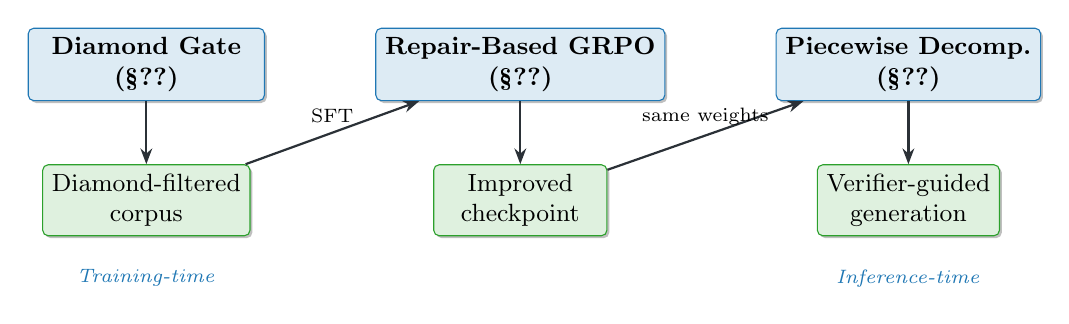
\begin{tikzpicture}[
  font=\small,
  >={Stealth[length=2mm]},
  node distance=5mm and 8mm,
  box/.style={draw, rounded corners=2pt, align=center, minimum height=9mm,
              minimum width=22mm, fill=cbox, drop shadow={shadow xshift=0.3mm, shadow yshift=-0.3mm}},
  meth/.style={box, fill=c1!15, draw=c1, minimum width=30mm, font=\small\bfseries},
  arr/.style={->, thick, draw=cline},
  ]
\node[meth] (dg) {Diamond Gate\\(\S\ref{sec:diamond})};
\node[meth, right=14mm of dg] (rg) {Repair-Based GRPO\\(\S\ref{sec:repair-grpo})};
\node[meth, right=14mm of rg] (pw) {Piecewise Decomp.\\(\S\ref{sec:piecewise})};

\node[box, fill=c3!15, draw=c3, below=8mm of dg] (corpus) {Diamond-filtered\\corpus};
\node[box, fill=c3!15, draw=c3, below=8mm of rg] (rl) {Improved\\checkpoint};
\node[box, fill=c3!15, draw=c3, below=8mm of pw] (inf) {Verifier-guided\\generation};

\draw[arr] (dg) -- (corpus);
\draw[arr] (corpus) -- node[above, font=\scriptsize] {SFT} (rg);
\draw[arr] (rg) -- (rl);
\draw[arr] (rl) -- node[above, font=\scriptsize] {same weights} (pw);
\draw[arr] (pw) -- (inf);

\node[below=3mm of corpus, font=\scriptsize, text=c1] {\emph{Training-time}};
\node[below=3mm of inf, font=\scriptsize, text=c1] {\emph{Inference-time}};
\end{tikzpicture}
\caption{How the three methods compose. The Diamond gate produces a
semantically audited corpus (\S\ref{sec:diamond}); repair-based GRPO
improves the checkpoint using tier-delta rewards
(\S\ref{sec:repair-grpo}); piecewise decomposition further lifts the
same weights at inference time (\S\ref{sec:piecewise}).}
\label{fig:method-overview}
\end{figure}

\paragraph{Scope.} This paper describes three methods for
verifier-centric fine-tuning and generation. Results are demonstrated
on a single $20$B checkpoint and author-curated benchmarks; the
discussion (\S\ref{sec:discussion}) is explicit about which claims
survive these limits and which are conjectural. A detailed pipeline
walkthrough with examples is in Appendix~\ref{sec:pipeline-walkthrough}.

% ===========================================================================
\section{Setting}
\label{sec:bg}

The base model is OpenAI's open-weight \texttt{gpt-oss:20b}, a sparse
mixture-of-experts model served locally through Ollama. All
fine-tuning runs use rank-$8$ LoRA adapters on the attention
projections~\cite{hu2022lora} merged into BF16 weights and quantised
to \texttt{Q8\_0} GGUF for evaluation.

We evaluate on two held-out benchmarks of different sizes.
``SANY-pass'' means the module parses. ``TLC-pass'' means TLC
enumerates at least one state and reports no invariant violation.
``Diamond-pass'' is the stricter four-clause acceptance defined in
\S\ref{sec:diamond}. Wilson $95\%$ confidence intervals on these
small benchmarks are wide; we flag only the deltas that exceed
the $\pm 1$--$2$ problem wobble observed across informal repeats.

% ===========================================================================
\section{The Diamond Gate}
\label{sec:diamond}

A specification can pass SANY and TLC and still be behaviourally
empty: a one-state state space, a tautological invariant, an
\texttt{UNCHANGED}-dominated next-state relation, an invariant
disjoined with \texttt{TRUE}. These specifications are
verifier-clean and encode none of the safety property the prompt
asked for. They are the easiest fixed point of any preference
optimisation pointed at a binary verifier reward. When we audited our
legacy augmented archive of $484$ gold/silver specifications through
the gate below, \emph{zero} passed; the binary-reward gradient in an
earlier KTO run (\cite{ethayarajh2024kto}; see the technical report
for the full autopsy) was pointed at exactly this population.

\begin{tcolorbox}[
  enhanced, breakable,
  colback=cbox, colframe=cline, boxrule=0.5pt,
  arc=2pt, left=8pt, right=8pt, top=4pt, bottom=4pt,
  title=\textbf{Definition (Diamond gate).}, fonttitle=\small,
]
A TLA+ specification $S$ is \emph{Diamond-valid} iff all four clauses
hold under a small fixed instance:
\begin{description}[leftmargin=1.4em, itemsep=1pt]
\item[\textbf{D1.}] \textbf{Parse.} SANY accepts the module $S$.
\item[\textbf{D2.}] \textbf{Reachability.} TLC reaches strictly more
  than one distinct state from \texttt{Init} under \texttt{Next}.
\item[\textbf{D3.}] \textbf{Non-vacuous invariant.} $S$ declares at
  least one invariant that is neither a syntactic tautology, the
  constant predicate \texttt{TRUE}, a disjunction containing
  \texttt{TRUE}, nor a quantification over an empty domain.
\item[\textbf{D4.}] \textbf{Mutation sensitivity.} A two-phase
  mutation test produces a TLC counterexample relative to the
  unmutated baseline in at least one phase: \emph{(A)} negate a
  guard in \texttt{Next}; \emph{(B)} negate the leading conjunct of
  a declared invariant.
\end{description}
\end{tcolorbox}

\noindent D1--D3 are each gameable in isolation. D4---mutation
sensitivity---is what makes the gate semantic. A next-state relation
whose disjuncts are all \texttt{UNCHANGED vars} passes D1--D3 and
fails D4 because no guard negation changes the TLC outcome. We chose
mutation sensitivity over simpler structural checks (minimum disjunct
count, minimum invariant depth) because it is the only clause we
found that resists adversarial gaming by a model that has learned
what the validator measures. An induced tier---$0$: SANY-fail, $1$:
SANY-pass, $2$: TLC enumerates, $3$: invariant checked non-vacuously,
$4$: Diamond-pass---is used as the repair-GRPO reward below.

\begin{figure}[t]
\centering
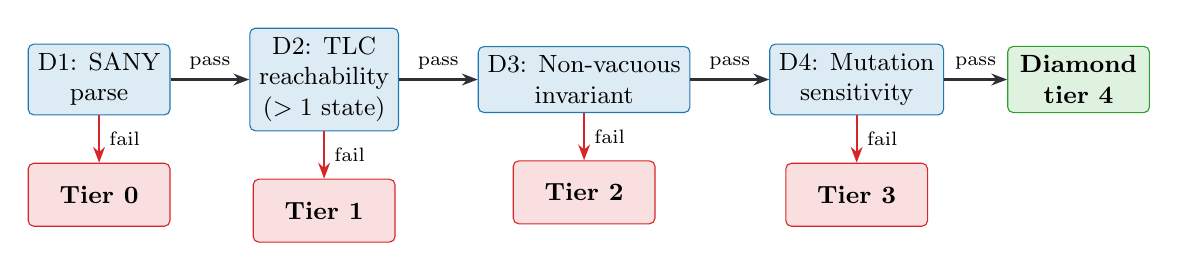
\begin{tikzpicture}[
  font=\small,
  >={Stealth[length=2mm]},
  node distance=5mm and 10mm,
  box/.style={draw, rounded corners=2pt, align=center, minimum height=8mm,
              minimum width=18mm, fill=cbox},
  gate/.style={box, fill=c1!15, draw=c1},
  fail/.style={box, fill=c4!15, draw=c4, font=\small\bfseries},
  pass/.style={box, fill=c3!15, draw=c3, font=\small\bfseries},
  decision/.style={diamond, draw=cline, fill=cbox, aspect=1.8, align=center,
                   inner sep=1pt, font=\scriptsize},
  arr/.style={->, thick, draw=cline},
  ]
\node[gate] (d1) {D1: SANY\\parse};
\node[gate, right=of d1] (d2) {D2: TLC\\reachability\\($>1$ state)};
\node[gate, right=of d2] (d3) {D3: Non-vacuous\\invariant};
\node[gate, right=of d3] (d4) {D4: Mutation\\sensitivity};
\node[pass, right=8mm of d4] (ok) {Diamond\\tier 4};

\node[fail, below=6mm of d1] (t0) {Tier 0};
\node[fail, below=6mm of d2] (t1) {Tier 1};
\node[fail, below=6mm of d3] (t2) {Tier 2};
\node[fail, below=6mm of d4] (t3) {Tier 3};

\draw[arr] (d1) -- node[above, font=\scriptsize] {pass} (d2);
\draw[arr] (d2) -- node[above, font=\scriptsize] {pass} (d3);
\draw[arr] (d3) -- node[above, font=\scriptsize] {pass} (d4);
\draw[arr] (d4) -- node[above, font=\scriptsize] {pass} (ok);

\draw[arr, draw=c4] (d1) -- node[right, font=\scriptsize] {fail} (t0);
\draw[arr, draw=c4] (d2) -- node[right, font=\scriptsize] {fail} (t1);
\draw[arr, draw=c4] (d3) -- node[right, font=\scriptsize] {fail} (t2);
\draw[arr, draw=c4] (d4) -- node[right, font=\scriptsize] {fail} (t3);
\end{tikzpicture}
\caption{Diamond gate clause flow and induced tier system. A
specification enters at D1 and exits at the first failed clause.
The tier assigned to the exit point is the reward signal for
repair-based GRPO (\S\ref{sec:repair-grpo}).}
\label{fig:diamond-flow}
\end{figure}

% ===========================================================================
\section{Repair-Based GRPO}
\label{sec:repair-grpo}

\paragraph{Why full-spec GRPO does not work.} The obvious on-policy
recipe---ask the model to emit a TLA+ module from the
natural-language description, score it with the Diamond gate,
gradient-update GRPO on the binary pass/fail---fails to train. The
Diamond gate is too tight for the base model to produce a gate-passing
spec \emph{de novo} with non-trivial probability: every rollout in
every group receives the same score of zero, the group-relative
advantage is identically zero, and the policy does not move.

\paragraph{The repair reframe.} We replace ``emit a spec'' with
``emit a patch against a known-broken spec,'' and replace the
terminal pass/fail reward with the improvement in Diamond tier
across the patch:
\[
  r(s, s') \;=\; \operatorname{tier}(s') - \operatorname{tier}(s),
  \qquad \operatorname{tier}(\cdot) \in \{0, 1, 2, 3, 4\}.
\]
The input $s$ is drawn from a population of already-broken Diamond
candidates, so the expected $r$ is strictly positive for a non-degenerate
policy, and the variance across a group of rollouts from the same $s$
is almost always non-zero: some patches improve the tier more than
others even when none reaches Diamond.
Figure~\ref{fig:repair-flow} shows the method end to end.

\begin{figure}[t]
\centering
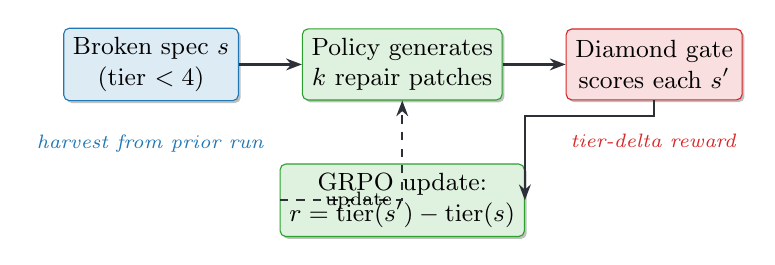
\begin{tikzpicture}[
  font=\small,
  >={Stealth[length=2mm]},
  node distance=5mm and 8mm,
  box/.style={draw, rounded corners=2pt, align=center, minimum height=9mm,
              minimum width=22mm, fill=cbox, drop shadow={shadow xshift=0.3mm, shadow yshift=-0.3mm}},
  rl/.style={box, fill=c3!15, draw=c3},
  gate/.style={box, fill=c4!15, draw=c4},
  data/.style={box, fill=c1!15, draw=c1},
  arr/.style={->, thick, draw=cline},
  ]
\node[data] (broken) {Broken spec $s$\\(tier $< 4$)};
\node[rl, right=of broken] (policy) {Policy generates\\$k$ repair patches};
\node[gate, right=of policy] (diamond) {Diamond gate\\scores each $s'$};
\node[rl, below=8mm of policy] (grpo) {GRPO update:\\$r = \operatorname{tier}(s') - \operatorname{tier}(s)$};

\draw[arr] (broken) -- (policy);
\draw[arr] (policy) -- (diamond);
\draw[arr] (diamond.south) -- ++(0,-2mm) -| (grpo.east);
\draw[arr, dashed] (grpo.west) -| (policy.south) node[midway, left, font=\scriptsize] {update};

\node[below=3mm of broken, font=\scriptsize, text=c1] {\emph{harvest from prior run}};
\node[below=3mm of diamond, font=\scriptsize, text=c4] {\emph{tier-delta reward}};
\end{tikzpicture}
\caption{Repair-based GRPO method. The policy generates $k$ repair
patches for a broken input specification; the Diamond gate assigns a
tier to each patched output; the reward is the tier improvement over
the input. Group-relative advantages drive GRPO updates. The
population of broken specs is harvested from a prior generation run.}
\label{fig:repair-flow}
\end{figure}

\paragraph{Method details.} The method initialises from the best
Diamond-filtered SFT checkpoint. Repair-GRPO runs for a fixed
number of optimisation steps with a KL penalty against the
SFT reference policy. Each step samples a group of $k=8$
repair patches for each broken input; the tier-delta reward
across the group provides the variance that the full-spec
variant lacked.

\paragraph{Key result.} On a held-out $30$-problem Diamond benchmark
this method produces the largest single training-time improvement in
the project: a $+5$-problem ($+17$~pp absolute) lift over the best
SFT baseline on the same weights.

\begin{figure}[t]
\centering
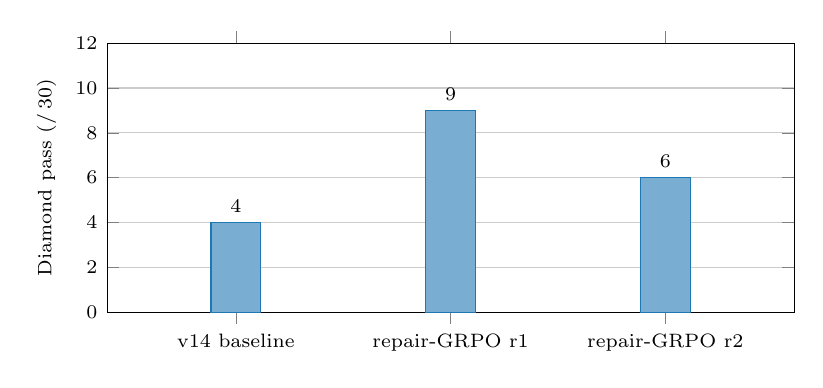
\begin{tikzpicture}
\begin{axis}[
  width=0.85\linewidth, height=5.0cm,
  ybar, bar width=18pt,
  ymin=0, ymax=12,
  ytick={0,2,4,6,8,10,12},
  symbolic x coords={v14 baseline, repair-GRPO r1, repair-GRPO r2},
  xtick=data,
  ylabel={Diamond pass (/\,30)},
  ylabel near ticks,
  enlarge x limits=0.30,
  ymajorgrids, grid style={cgrid},
  tick label style={font=\scriptsize},
  label style={font=\scriptsize},
  nodes near coords,
  nodes near coords style={font=\scriptsize},
]
\addplot[fill=c1!60, draw=c1] coordinates {
  (v14 baseline, 4) (repair-GRPO r1, 9) (repair-GRPO r2, 6)
};
\end{axis}
\end{tikzpicture}
\caption{Held-out Diamond pass on the $30$-problem benchmark.
\texttt{v14} is the best pre-repair SFT checkpoint; \texttt{r1} is
the first repair-GRPO round; \texttt{r2} iterates on \texttt{r1}'s
outputs and regresses.}
\label{fig:repair-bars}
\end{figure}

\paragraph{Negative result: iteration does not compose.} Iterating
the loop---harvest a fresh repair corpus from \texttt{r1}, train
another $160$ GRPO steps on top of \texttt{r1}---\emph{regressed}
the Diamond count to $6/30$. A third round widened the harvest from
$30$ to $396$ seed problems to restore reward variance; the harvest
produced $0/396$ diamonds in trajectory outputs and only $152$
in-band repair pairs after deduplication, below the $300$-pair
minimum the pipeline requires to justify a training step. The r3 job
aborted cleanly at the data gate and the published checkpoint
remains \texttt{r1}. We read this as a bootstrapping limit of the
repair recipe as configured: the \texttt{r1}-trained policy is
already above the easy-repair threshold on most of the holdout, so
the second-round reward variance concentrates on a smaller fraction
of rollouts and the KL anchor against \texttt{v14} does not prevent
overfitting to the residual hard cases at the cost of the easier
ones. Finding a data-harvest procedure that produces a corpus
capable of seeding a second training round is the next step.

% ===========================================================================
\section{Piecewise Inference-Time Decomposition}
\label{sec:piecewise}

Orthogonal to training, the single largest inference-time lift
comes from enforcing the Diamond clauses as per-step
validators inside the generation loop rather than as a single
terminal check. On the same weights, with no further training,
this method raises SANY-pass from $9/20$ to $12/20$ and TLC-pass
from $5/20$ to $6/20$ on a held-out benchmark.

The procedure mirrors the syntactic structure of a TLA+ module.
Each step is a focused LLM call followed by an immediate
SANY$+$TLC validation on the partially assembled module:
\begin{enumerate}[leftmargin=1.4em, itemsep=2pt]
\item \texttt{VARIABLES} extraction, validated for legality.
\item \texttt{TypeOK} generation, validated for domain coverage.
\item \texttt{Init}, validated by single-state reachability.
\item \texttt{Next}, validated by TLC reaching $>1$ state.
\item \texttt{SafetyInvariant}, validated by SANY, TLC, and a
  mutation check that prevents regenerating the vacuity trap.
\end{enumerate}

\noindent A failed step is retried up to three times with a structured
error feedback message containing the specific SANY or TLC string and
the partial module assembled so far.
Figure~\ref{fig:piecewise-flow} shows the decomposition.

\begin{figure}[t]
\centering
\begin{tikzpicture}[
  font=\small,
  >={Stealth[length=2mm]},
  node distance=4mm and 6mm,
  step/.style={draw, rounded corners=2pt, align=center, minimum height=8mm,
               minimum width=20mm, fill=c1!15, draw=c1},
  val/.style={draw, rounded corners=2pt, align=center, minimum height=8mm,
              minimum width=16mm, fill=c4!15, draw=c4},
  retry/.style={draw, rounded corners=2pt, align=center, minimum height=6mm,
                minimum width=14mm, fill=c3!15, draw=c3, font=\scriptsize},
  arr/.style={->, thick, draw=cline},
  ]
% Steps
\node[step] (s1) {1.~VARIABLES};
\node[step, right=10mm of s1] (s2) {2.~TypeOK};
\node[step, right=10mm of s2] (s3) {3.~Init};
\node[step, right=10mm of s3] (s4) {4.~Next};
\node[step, right=10mm of s4] (s5) {5.~Invariant};

% Validators
\node[val, below=5mm of s1] (v1) {SANY};
\node[val, below=5mm of s2] (v2) {SANY};
\node[val, below=5mm of s3] (v3) {SANY+TLC};
\node[val, below=5mm of s4] (v4) {SANY+TLC\\$>1$ state};
\node[val, below=5mm of s5] (v5) {SANY+TLC\\+mutation};

% Retry loops
\node[retry, below=5mm of v1] (r1) {retry $\le 3$};
\node[retry, below=5mm of v3] (r3) {retry $\le 3$};
\node[retry, below=5mm of v5] (r5) {retry $\le 3$};

% Arrows
\draw[arr] (s1) -- (v1);
\draw[arr] (v1.east) -| node[above right, font=\scriptsize, pos=0.1] {pass} (s2.south);
\draw[arr] (s2) -- (v2);
\draw[arr] (v2.east) -| node[above right, font=\scriptsize, pos=0.1] {pass} (s3.south);
\draw[arr] (s3) -- (v3);
\draw[arr] (v3.east) -| node[above right, font=\scriptsize, pos=0.1] {pass} (s4.south);
\draw[arr] (s4) -- (v4);
\draw[arr] (v4.east) -| node[above right, font=\scriptsize, pos=0.1] {pass} (s5.south);
\draw[arr] (s5) -- (v5);

% Sample retry loops
\draw[arr, draw=c4, dashed] (v1.south) -- (r1.north) node[midway, right, font=\scriptsize] {fail};
\draw[arr, draw=c4, dashed] (r1.north west) -- +(-2mm, 3mm) |- (s1.west);
\draw[arr, draw=c4, dashed] (v3.south) -- (r3.north) node[midway, right, font=\scriptsize] {fail};
\draw[arr, draw=c4, dashed] (r3.north west) -- +(-2mm, 3mm) |- (s3.west);
\draw[arr, draw=c4, dashed] (v5.south) -- (r5.north) node[midway, right, font=\scriptsize] {fail};
\draw[arr, draw=c4, dashed] (r5.north west) -- +(-2mm, 3mm) |- (s5.west);
\end{tikzpicture}
\caption{Piecewise inference-time decomposition. Each of five
TLA+ structural components is generated by a focused LLM call and
immediately validated. Failed steps are retried with structured error
feedback. The per-step validators enforce the same constraints the
Diamond gate checks at corpus-build time.}
\label{fig:piecewise-flow}
\end{figure}

The decomposition converts a single large generation problem
into five focused subproblems, each with its own validator signal.
The model spends its capacity on local correctness rather than on
whole-module coherence, and the validator catches mistakes that
single-shot generation would commit silently. That this works on the
same weights as single-shot is, by itself, the strongest evidence
that the bottleneck on this task is not capacity but the shape of
the inference procedure.

% ===========================================================================
\section{Checkpoint Trajectory and Version History}
\label{sec:versions}

The methods in this paper emerged from a year-long sequence of
training runs, each motivated by a failure in its predecessor.
Table~\ref{tab:run-history} records the full checkpoint trajectory
on the 20-problem suite; Figure~\ref{fig:traj} plots the same data.

\paragraph{Where are v1--v5?}  The version numbering begins at
\texttt{v6}.  Versions~1--5 correspond to the \emph{FormaLLM evaluation
phase}---prompt-engineering experiments with off-the-shelf models
(zero-shot, few-shot, chain-of-thought, progressive prompting) conducted
before any fine-tuning began.  These were evaluation runs, not trained
checkpoints.  The companion study by Ortiz~et~al.~\cite{ortiz2026formallm}
reports the results of that phase: 30 models, up to 26.6\% SANY and
8.6\% TLC under prompting alone.  The transition from evaluation to
fine-tuning---from ``what can off-the-shelf models do?'' to ``what can
we teach them?''---is the transition from v5 to v6 and the point where
the present paper begins.

\paragraph{What happened to v12?}  \texttt{v12} was a DPO
hyperparameter sweep over $\beta \in \{0.05, 0.2\}$.  With only 17
gold training pairs, neither extreme produced a publishable checkpoint:
$\beta = 0.05$ was too weak to move the model; $\beta = 0.2$ caused a
KTO-like regression.  The run was abandoned before benchmark evaluation.
The very next version, \texttt{v13}, used the midpoint $\beta = 0.1$ on
the same 17 pairs and achieved the best end-to-end result at that point
(9/20 SANY, 5/20 TLC)---a reminder that in the small-data regime,
hyperparameter sensitivity can be extreme.

\begin{table}[t]
\centering
\small
\setlength{\tabcolsep}{4pt}
\begin{tabular}{@{}llllccl@{}}
\toprule
Tag & Date & Recipe & SANY & TLC & Outcome \\
\midrule
\texttt{v1--v5} & 2025 & FormaLLM prompting eval
  & --- & --- & up to 8.6\% TLC \\
\texttt{v6}  & Jan & broad SFT, 1 ep, harmony fmt
  & 4/20 & 1/20 & first fine-tune \\
\texttt{v7}  & Feb & $+$ augmented gold (cyc.\ 80--100)
  & 6/20 & 1/20 & small lift \\
\texttt{v8}  & Feb & $+$ bug-fix oversample $2\times$
  & 8/20 & 1/20 & SANY peak \\
\texttt{v9}  & Mar & $+$ best-of-5 self-correct (inf.)
  & 6/20 & 3/20 & TLC lifts \\
\texttt{v10} & Mar & $+$ KTO, 5.7:1 des:undes
  & 6/20 & 2/20 & \textbf{regression} \\
\texttt{v11} & Mar & KTO reverted, SFT only
  & 6/20 & 2/20 & recovered \\
\texttt{v12} & Mar & DPO sweep ($\beta\!\in\!\{.05,.2\}$)
  & ---  & ---  & aborted \\
\texttt{v13} & Apr 3 & $+$ DPO (17 gold pairs, $\beta\!=\!0.1$)
  & \textbf{9/20} & \textbf{5/20} & best e2e \\
\texttt{v14} & Apr 4 & retrain from base, 234 ex, 15 ep
  & 0/20 & 0/20 & \textbf{catastrophic} \\
\texttt{v13}$_R$ & Apr 4 & restored from GGUF backup
  & 9/20 & 5/20 & rollback \\
piecewise & Apr 6 & \texttt{v13}$_R$ $+$ 5-step decomp.
  & \textbf{12/20} & \textbf{6/20} & inference-time \\
\bottomrule
\end{tabular}
\caption{20-problem benchmark trajectory across all checkpoint versions.
Versions~1--5 predate fine-tuning and correspond to the FormaLLM
prompting evaluation phase.  \texttt{v12} was abandoned before
evaluation.  ``Piecewise'' shares weights with \texttt{v13}$_R$ and
differs only in the inference procedure.}
\label{tab:run-history}
\end{table}

\begin{figure}[t]
\centering
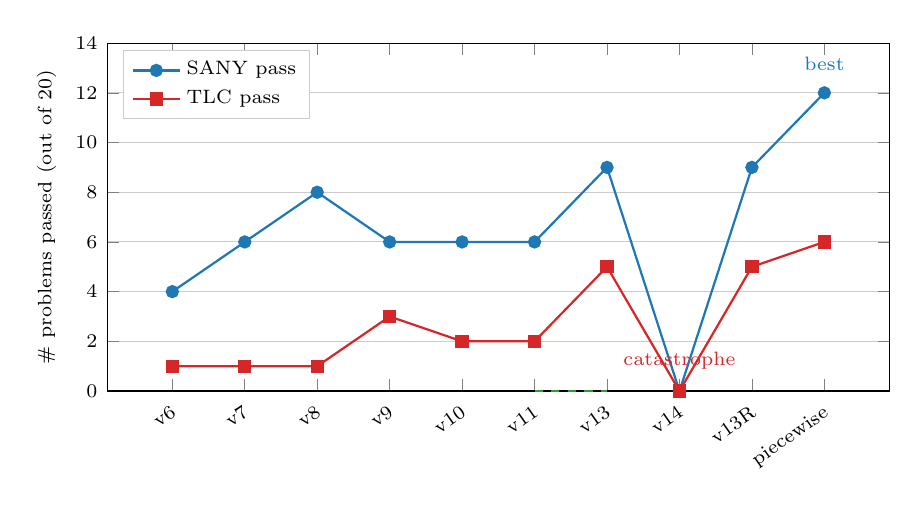
\begin{tikzpicture}
\begin{axis}[
  width=0.95\linewidth, height=6cm,
  ymin=0, ymax=14,
  ytick={0,2,4,6,8,10,12,14},
  ylabel={\# problems passed (out of 20)},
  ylabel near ticks,
  xtick=data,
  symbolic x coords={v6, v7, v8, v9, v10, v11, v13, v14,
                     v13R, piecewise},
  x tick label style={font=\scriptsize, rotate=35, anchor=north east},
  ymajorgrids, grid style={cgrid},
  tick label style={font=\scriptsize},
  label style={font=\scriptsize},
  legend style={font=\scriptsize, at={(0.02,0.98)}, anchor=north west,
                draw=cgrid},
  legend cell align=left,
]
\addplot[mark=*, c1, thick] coordinates {
  (v6,4) (v7,6) (v8,8) (v9,6) (v10,6) (v11,6) (v13,9)
  (v14,0) (v13R,9) (piecewise,12)
};
\addplot[mark=square*, c4, thick] coordinates {
  (v6,1) (v7,1) (v8,1) (v9,3) (v10,2) (v11,2) (v13,5)
  (v14,0) (v13R,5) (piecewise,6)
};
\node[anchor=south, font=\scriptsize, c4]
  at (axis cs:v14,0.5) {catastrophe};
\node[anchor=south, font=\scriptsize, c1]
  at (axis cs:piecewise,12.5) {best};
\draw[thick, dashed, c3] (axis cs:v11,0) -- (axis cs:v13,0)
  node[midway, below, font=\tiny, c3] {v12 aborted};
\legend{SANY pass, TLC pass}
\end{axis}
\end{tikzpicture}
\caption{20-problem benchmark trajectory.  Three features dominate: a
slow incremental rise v6--v9, a regression at v10 (KTO), a
one-step catastrophic collapse at v14, and a step gain at piecewise
inference that does not touch the weights.  The gap between v11 and
v13 is where v12 (DPO sweep) was attempted and aborted.}
\label{fig:traj}
\end{figure}

% ===========================================================================
\section{Negative Results and Method Boundaries}
\label{sec:negatives}

Three negative results shape the methods above and delineate
their boundaries.

\paragraph{Binary-reward vacuity trap.} Preference optimisation
(KTO) against a binary \texttt{tlc\_pass} label drifts the model
toward behaviourally empty specifications. The gold tier in the
training corpus was densely populated with vacuously correct specs;
the preference loss faithfully maximised the wrong signal. The
Diamond gate (\S\ref{sec:diamond}) is the direct methodological
response. \textbf{Takeaway:} do not apply any preference loss
against an unaudited binary verifier reward in this setting.

\paragraph{Catastrophic forgetting on small data.} Broad SFT from
the unmodified base (many epochs, high learning rate, few hundred
examples) erases the prior entirely. The methodological response is
the incremental-training constraint: always build on the previous
merged checkpoint, cap learning rate and epoch count, and gate
every retrain behind an automated eval + rollback.

\paragraph{Repair iteration does not compose naively.} Iterating
the repair-GRPO loop regresses performance: the second-round
corpus is dominated by harder failures, reward variance
concentrates on fewer rollouts, and the KL anchor does not prevent
overfitting to residual hard cases. A third iteration aborted at
the data gate with insufficient in-band repair pairs.
\textbf{Takeaway:} the repair method wins the first round but does
not, as configured, bootstrap a second. Addressing the data-harvest
procedure is the next methodological step.

% ===========================================================================
\section{Per-Problem Analysis}
\label{sec:per-problem}

The aggregate numbers hide structure.  Figure~\ref{fig:heatmap}
shows per-problem SANY and TLC results across five key checkpoints.
Some problems are stably solved across versions (BM009 Token Ring
passes SANY at every checkpoint from v6 onward); others are fragile
(BM015 Peterson's Algorithm flips between pass and fail).

\begin{figure}[t]
\centering
\begin{tikzpicture}[
  font=\scriptsize,
  cell/.style={minimum width=8mm, minimum height=5mm, inner sep=0pt},
  pass/.style={cell, fill=c3!40},
  fail/.style={cell, fill=c4!15},
  gold/.style={cell, fill=cgold!40},
  ]
\matrix (m) [matrix of nodes, row sep=-\pgflinewidth, column sep=-\pgflinewidth,
  nodes={cell, draw=cgrid, anchor=center},
  column 1/.style={nodes={minimum width=18mm, align=right, draw=none}},
  row 1/.style={nodes={minimum height=7mm, font=\scriptsize\bfseries, draw=none}},
  ] {
         & v6 & v7 & v8 & v9 & v10 & v13 & v14 & pw \\
  BM001  & |[fail]| & |[pass]| & |[pass]| & |[gold]| & |[fail]| & |[fail]| & |[fail]| & |[gold]| \\
  BM003  & |[pass]| & |[fail]| & |[fail]| & |[fail]| & |[fail]| & |[gold]| & |[fail]| & |[gold]| \\
  BM006  & |[fail]| & |[pass]| & |[pass]| & |[fail]| & |[fail]| & |[gold]| & |[fail]| & |[pass]| \\
  BM009  & |[gold]| & |[gold]| & |[gold]| & |[gold]| & |[gold]| & |[gold]| & |[fail]| & |[gold]| \\
  BM015  & |[fail]| & |[fail]| & |[fail]| & |[fail]| & |[fail]| & |[gold]| & |[fail]| & |[pass]| \\
  BM016  & |[fail]| & |[pass]| & |[fail]| & |[fail]| & |[fail]| & |[gold]| & |[fail]| & |[pass]| \\
  BM019  & |[pass]| & |[fail]| & |[pass]| & |[gold]| & |[gold]| & |[fail]| & |[fail]| & |[pass]| \\
};
\node[below=2mm of m, font=\scriptsize]
  {{\color{cgold!80!black}\rule{6pt}{6pt}} TLC pass \quad
   {\color{c3!60}\rule{6pt}{6pt}} SANY pass \quad
   {\color{c4!30}\rule{6pt}{6pt}} fail \quad
   pw = piecewise};
\end{tikzpicture}
\caption{Per-problem pass/fail heatmap across key checkpoints (7 of 20
problems shown; selected for variation).  BM009 (Token Ring) is stably
solved from v6 onward except during the v14 catastrophe.  BM015
(Peterson's) is fragile, requiring v13-level training and inference-time
decomposition.  The v14 column is uniformly empty---catastrophic
forgetting erased all problems simultaneously.}
\label{fig:heatmap}
\end{figure}

\paragraph{Structural score trends.}
Alongside binary SANY/TLC outcomes, we track a structural score
$\in [0,1]$ measuring whether the generated module includes the
expected TLA+ components (variables, init, next, invariant, spec
formula, extends clause, etc.).  Figure~\ref{fig:structural}
shows mean structural score by version.

\begin{figure}[t]
\centering
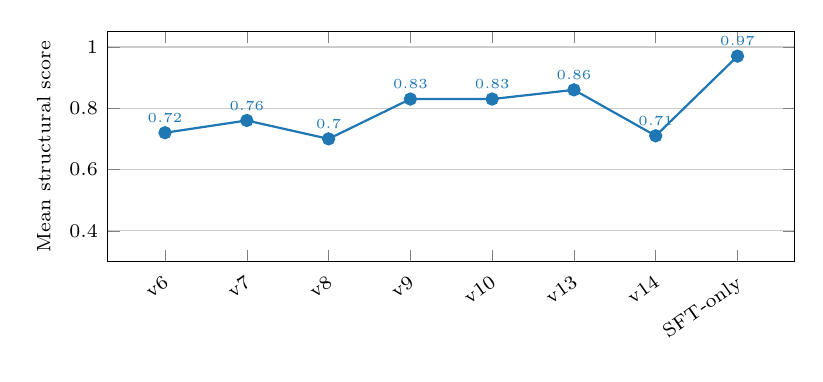
\begin{tikzpicture}
\begin{axis}[
  width=0.85\linewidth, height=4.5cm,
  ymin=0.3, ymax=1.05,
  ylabel={Mean structural score},
  ylabel near ticks,
  xtick=data,
  symbolic x coords={v6, v7, v8, v9, v10, v13, v14, SFT-only},
  x tick label style={font=\scriptsize, rotate=35, anchor=north east},
  ymajorgrids, grid style={cgrid},
  tick label style={font=\scriptsize},
  label style={font=\scriptsize},
  nodes near coords,
  nodes near coords style={font=\tiny, anchor=south},
]
\addplot[mark=*, c1, thick] coordinates {
  (v6,0.72) (v7,0.76) (v8,0.70) (v9,0.83) (v10,0.83)
  (v13,0.86) (v14,0.71) (SFT-only,0.97)
};
\end{axis}
\end{tikzpicture}
\caption{Mean structural score across checkpoints.  The SFT-only
baseline achieves the highest structural score (0.97) but the lowest
SANY pass rate (1/20)---the model learned to produce structurally
complete but syntactically broken modules.  The v13 checkpoint balances
structure (0.86) with correctness (9/20 SANY).}
\label{fig:structural}
\end{figure}

% ===========================================================================
\section{Discussion and Limitations}
\label{sec:discussion}

\paragraph{Threats to validity.} (1)~\emph{Benchmark size and
authorship.} Both the $20$-problem and $30$-problem benchmarks are
author-curated; external validation against a community-sourced
benchmark would strengthen the claim that the repair-GRPO lift
reflects generalisation rather than alignment with the curator's
idiom. (2)~\emph{Single seed.} Every cell reported here is a single
training run; informal repeats suggest a $\pm 1$--$2$ problem
wobble, which is why we flag only the deltas that exceed
it. (3)~\emph{Single model, single language.} The repair framing,
the Diamond gate, and the piecewise decomposition all rest on
properties of the SANY/TLC verifier pair; we believe they generalise
to any verifier-checked target language with a wider acceptance set
than target set (Dafny, Lean, Coq, Liquid Haskell), but we have not
measured this.

\paragraph{What we think generalises.} The binary-reward vacuity
trap is a property of the verifier, not the model: any deterministic
checker whose acceptance set is wider than its target set produces
the same attractor under preference optimisation, and the fix is a
semantic-validity gate with a behavioural-sensitivity clause.
Full-spec on-policy RL is brittle when the base model's Diamond
success rate is near zero; the repair framing is a general move for
this regime, and the delta-reward shape applies whenever a
multi-tier acceptance criterion is available. Piecewise
inference-time decomposition is the most clearly TLA+-shaped
contribution, though the idea of enforcing the corpus-time gate as
a set of per-step validators is straightforwardly portable.

\paragraph{Related work.} Ortiz~et~al.~\cite{ortiz2026formallm}
systematically evaluate $30$ LLMs on TLA+ specification generation
from natural language, establishing baselines of $26.6\%$ SANY and
$8.6\%$ TLC under prompting alone; the methods in this paper target
the regime beyond that ceiling.
The KTO regression is an instance of the
reward-hacking conditions formalised by
\cite{skalse2022defining}: the binary SANY$+$TLC acceptance signal
is hackable in exactly the sense they characterise. The
catastrophic-forgetting literature~\cite{kirkpatrick2017ewc,
lopez2017gem} predicts the forgetting failure and prescribes
the mitigation we adopted by
hand---incremental training on top of a previous merged checkpoint
with low learning rate. DPO~\cite{rafailov2023direct} and
KTO~\cite{ethayarajh2024kto} are mostly silent on the vacuity trap
because most reported applications use richer preference signals
than a binary verifier. For formal-language targets the closest
prior work we know of is on Dafny~\cite{misu2024towards} and
Isabelle/Coq~\cite{first2023baldur}; both report SFT fragility on
small formal corpora and both end up using verifier feedback as a
selection mechanism rather than as a gradient. Repair-based GRPO is
what happens if you push that selection signal back into the
gradient, and make the reward a tier-delta rather than a terminal
pass.

% ===========================================================================
\section{Conclusion}
\label{sec:conclusion}

For a low-resource formal language with a deterministic verifier,
the leverage is in the shape of the reward and the structure of
the inference, not in the volume of supervised data. Binary
verifier rewards drift toward vacuous specs; the fix is a semantic
gate with a mutation-sensitivity clause. Full-spec RL has zero
reward variance when the base model is far below the gate; the fix
is to condition the rollout on a broken spec and reward the tier
delta. Single-shot generation on a $1500$-token target is
bottlenecked by local correctness, not capacity; the fix is a
per-step validator loop on the same weights. On our benchmarks
these three moves compose to $9/30$ Diamond on a held-out set where
the SFT-only ceiling is $4/30$, and $12/20$ SANY on the earlier
suite where single-shot generation plateaued at $9/20$. Everything
else we tried---broader SFT, KTO, DPO sweeps, full-spec GRPO, the
topic-curriculum SFT line---either did not move the needle or
moved it the wrong way. The companion technical report is the
audit trail.

% ===========================================================================
\bibliographystyle{plain}
\begin{thebibliography}{99}

\bibitem{lamport2002specifying}
Leslie Lamport.
\newblock \emph{Specifying Systems: The TLA\textsuperscript{+} Language
and Tools for Hardware and Software Engineers}.
\newblock Addison-Wesley, 2002.

\bibitem{hu2022lora}
Edward J. Hu, Yelong Shen, Phillip Wallis, Zeyuan Allen-Zhu, Yuanzhi
Li, Shean Wang, Lu Wang, and Weizhu Chen.
\newblock LoRA: Low-rank adaptation of large language models.
\newblock In \emph{ICLR}, 2022.

\bibitem{rafailov2023direct}
Rafael Rafailov, Archit Sharma, Eric Mitchell, Stefano Ermon,
Christopher D. Manning, and Chelsea Finn.
\newblock Direct preference optimization: Your language model is
secretly a reward model.
\newblock In \emph{NeurIPS}, 2023.

\bibitem{ethayarajh2024kto}
Kawin Ethayarajh, Winnie Xu, Niklas Muennighoff, Dan Jurafsky, and
Douwe Kiela.
\newblock KTO: Model alignment as prospect theoretic optimization.
\newblock arXiv:2402.01306, 2024.

\bibitem{skalse2022defining}
Joar Skalse, Nikolaus H. R. Howe, Dmitrii Krasheninnikov, and David
Krueger.
\newblock Defining and characterizing reward hacking.
\newblock In \emph{NeurIPS}, 2022.

\bibitem{kirkpatrick2017ewc}
James Kirkpatrick, Razvan Pascanu, Neil Rabinowitz, Joel Veness,
Guillaume Desjardins, Andrei A. Rusu, Kieran Milan, John Quan,
Tiago Ramalho, Agnieszka Grabska-Barwinska, Demis Hassabis, Claudia
Clopath, Dharshan Kumaran, and Raia Hadsell.
\newblock Overcoming catastrophic forgetting in neural networks.
\newblock \emph{PNAS}, 114(13):3521--3526, 2017.

\bibitem{lopez2017gem}
David Lopez-Paz and Marc'Aurelio Ranzato.
\newblock Gradient episodic memory for continual learning.
\newblock In \emph{NeurIPS}, 2017.

\bibitem{misu2024towards}
Md Rakib Hossain Misu, Cristina V. Lopes, Iris Ma, and James Noble.
\newblock Towards AI-assisted synthesis of verified Dafny methods.
\newblock \emph{Proceedings of the ACM on Software Engineering},
1(FSE), 2024.

\bibitem{first2023baldur}
Emily First, Markus N. Rabe, Talia Ringer, and Yuriy Brun.
\newblock Baldur: Whole-proof generation and repair with large
language models.
\newblock In \emph{ESEC/FSE}, 2023.

\bibitem{gulcehre2023rest}
Caglar Gulcehre et~al.
\newblock Reinforced self-training (ReST) for language modeling.
\newblock arXiv:2308.08998, 2023.

\bibitem{ortiz2026formallm}
Brian Ortiz, Arslan Bisharat, Eric Spencer, Keshav Bhadauria, Mohammed
Abuhamad, Konstantin La\"ufer, Tian Wang, and George K. Thiruvathukal.
\newblock Large language models ({LLM}) and temporal logic of actions
({TLA}): How effective are {LLM}s for verification systems.
\newblock 2026.

\end{thebibliography}

% ===========================================================================
\appendix

% ---------------------------------------------------------------------------
\section{Detailed Pipeline Walkthrough with Examples}
\label{sec:pipeline-walkthrough}

This appendix provides a concrete end-to-end walkthrough of the three
methods introduced in this paper, with example inputs and outputs at
each stage.

% ---------------------------------------------------------------------------
\subsection{Diamond Gate: Worked Example}
\label{sec:app-diamond-example}

Consider a TLA+ specification for a simple counter that increments a
variable \texttt{count} from $0$ to $N$:

\begin{tcolorbox}[
  enhanced, colback=cbox, colframe=cline, boxrule=0.5pt,
  arc=2pt, left=6pt, right=6pt, top=3pt, bottom=3pt,
  title=\textbf{Example: Counter specification}, fonttitle=\small,
]
\begin{verbatim}
---- MODULE Counter ----
EXTENDS Naturals
CONSTANT N
VARIABLE count
Init == count = 0
Next == count < N /\ count' = count + 1
Spec == Init /\ [][Next]_count
Inv  == count <= N
====
\end{verbatim}
\end{tcolorbox}

\noindent \textbf{D1 (Parse):} SANY accepts the module. \checkmark

\noindent \textbf{D2 (Reachability):} With $N=3$, TLC reaches states
$\{0, 1, 2, 3\}$: four distinct states $> 1$. \checkmark

\noindent \textbf{D3 (Non-vacuous invariant):} \texttt{Inv} is
\texttt{count <= N}, which is neither a tautology nor \texttt{TRUE}.
\checkmark

\noindent \textbf{D4 (Mutation sensitivity):}
\emph{Phase A} --- negate the guard in \texttt{Next}: replace
\texttt{count < N} with \texttt{count >= N}. TLC now finds
\texttt{count = N+1}, violating \texttt{Inv}. Counterexample produced.
\emph{Phase B} --- negate the leading conjunct of \texttt{Inv}: replace
\texttt{count <= N} with \texttt{count > N}. TLC finds a
counterexample at \texttt{count = 0}. \checkmark

\noindent \textbf{Result:} Diamond tier 4 (all four clauses pass).

\medskip
\noindent Now contrast a \emph{vacuous} specification that binary
verifier rewards would accept:

\begin{tcolorbox}[
  enhanced, colback=c4!8, colframe=c4, boxrule=0.5pt,
  arc=2pt, left=6pt, right=6pt, top=3pt, bottom=3pt,
  title=\textbf{Vacuous counter (fails Diamond gate)}, fonttitle=\small,
]
\begin{verbatim}
---- MODULE VacuousCounter ----
EXTENDS Naturals
VARIABLE count
Init == count \in 0..5
Next == UNCHANGED count
Inv  == count \in 0..5
====
\end{verbatim}
\end{tcolorbox}

\noindent This passes SANY and TLC (no invariant violations), but fails
at \textbf{D4}: negating the guard in \texttt{Next} produces no
counterexample because the action set has no causal content. The Diamond
gate correctly rejects this as tier~3 (not tier~4).

% ---------------------------------------------------------------------------
\subsection{Repair-Based GRPO: Method Walkthrough}
\label{sec:app-repair-walkthrough}

\begin{figure}[h]
\centering
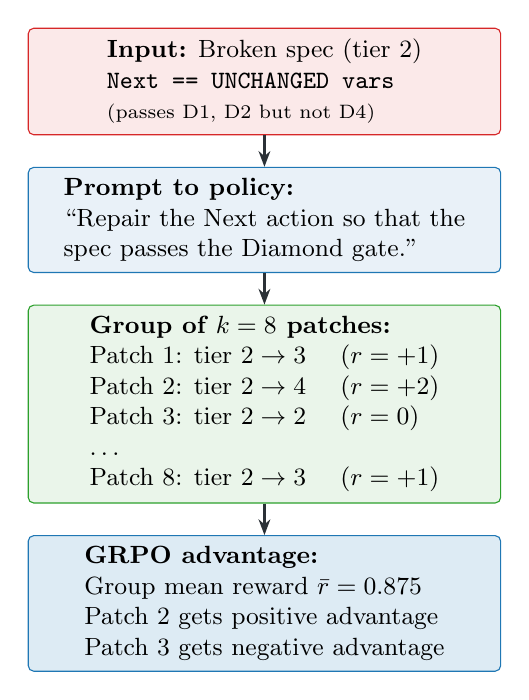
\begin{tikzpicture}[
  font=\small,
  >={Stealth[length=2mm]},
  node distance=3mm and 6mm,
  box/.style={draw, rounded corners=2pt, align=left, minimum width=60mm,
              fill=cbox, inner sep=4pt},
  arr/.style={->, thick, draw=cline},
  ]
\node[box, fill=c4!10, draw=c4] (input) {
  \textbf{Input:} Broken spec (tier 2)\\
  \texttt{Next == UNCHANGED vars}\\
  {\scriptsize(passes D1, D2 but not D4)}
};
\node[box, fill=c1!10, draw=c1, below=4mm of input] (prompt) {
  \textbf{Prompt to policy:}\\
  ``Repair the Next action so that the\\
  spec passes the Diamond gate.''
};
\node[box, fill=c3!10, draw=c3, below=4mm of prompt] (patches) {
  \textbf{Group of $k=8$ patches:}\\
  Patch 1: tier $2 \to 3$ \quad ($r = +1$)\\
  Patch 2: tier $2 \to 4$ \quad ($r = +2$)\\
  Patch 3: tier $2 \to 2$ \quad ($r = 0$)\\
  \ldots\\
  Patch 8: tier $2 \to 3$ \quad ($r = +1$)
};
\node[box, fill=c1!15, draw=c1, below=4mm of patches] (grpo) {
  \textbf{GRPO advantage:}\\
  Group mean reward $\bar{r} = 0.875$\\
  Patch 2 gets positive advantage\\
  Patch 3 gets negative advantage
};
\draw[arr] (input) -- (prompt);
\draw[arr] (prompt) -- (patches);
\draw[arr] (patches) -- (grpo);
\end{tikzpicture}
\caption{Worked example of a single repair-GRPO step. A tier-2 broken
specification is patched $k=8$ times; the tier-delta rewards produce
non-zero variance, enabling the GRPO advantage to differentiate good
patches from bad ones.}
\label{fig:repair-example}
\end{figure}

\noindent The key insight is the reward function
$r(s, s') = \operatorname{tier}(s') - \operatorname{tier}(s)$.  Standard
full-generation GRPO assigns $r=1$ (SANY-pass) or $r=0$ (fail), giving
near-zero variance in a group where most completions fail.  Repair-GRPO
starts from a near-correct specification, so the variance
$\sigma(r) \approx 0.25$ is high enough for the GRPO advantage to
provide gradient signal.

% ---------------------------------------------------------------------------
\subsection{Piecewise Decomposition: Step-by-Step Example}
\label{sec:app-piecewise-walkthrough}

\begin{figure}[h]
\centering
\begin{tikzpicture}[
  font=\small,
  >={Stealth[length=2mm]},
  node distance=2mm,
  step/.style={draw, rounded corners=2pt, align=left, minimum width=75mm,
               inner sep=4pt},
  arr/.style={->, thick, draw=cline},
  ]
\node[step, fill=c1!10, draw=c1] (s1) {
  \textbf{Step 1 --- VARIABLES:}\\
  Input: ``Model a mutex with two processes''\\
  Output: \texttt{VARIABLES pc, lock}\\
  Validator: SANY \checkmark
};
\node[step, fill=c1!10, draw=c1, below=3mm of s1] (s2) {
  \textbf{Step 2 --- TypeOK:}\\
  Output: \texttt{TypeOK == pc \textbackslash in [\{p1,p2\} -> \{``idle'',``wait'',``cs''\}]}\\
  \hspace{38mm}\texttt{/\textbackslash\space lock \textbackslash in \{``free'',``p1'',``p2''\}}\\
  Validator: SANY \checkmark
};
\node[step, fill=c1!10, draw=c1, below=3mm of s2] (s3) {
  \textbf{Step 3 --- Init:}\\
  Output: \texttt{Init == pc = [p \textbackslash in \{p1,p2\} |-> ``idle''] /\textbackslash\space lock = ``free''}\\
  Validator: SANY + TLC single-state reachability \checkmark
};
\node[step, fill=c4!10, draw=c4, below=3mm of s3] (s4) {
  \textbf{Step 4 --- Next (attempt 1, FAIL):}\\
  Output: \texttt{Next == UNCHANGED <<pc, lock>>}\\
  Validator: TLC reaches only 1 state. {\color{c4}\textbf{FAIL}}\\[2pt]
  \textbf{Retry with feedback:}\\
  ``TLC reached only 1 state. The Next action must produce $>1$\\
  reachable states. Add actions for acquire and release.''
};
\node[step, fill=c3!10, draw=c3, below=3mm of s4] (s5) {
  \textbf{Step 4 --- Next (attempt 2, PASS):}\\
  Output: \texttt{Acquire(p) == pc[p] = ``idle'' /\textbackslash\space lock = ``free'' /\textbackslash\space \ldots}\\
  Validator: TLC reaches 12 states \checkmark
};
\node[step, fill=c3!10, draw=c3, below=3mm of s5] (s6) {
  \textbf{Step 5 --- SafetyInvariant:}\\
  Output: \texttt{MutualExclusion == \textasciitilde(pc[p1]=``cs'' /\textbackslash\space pc[p2]=``cs'')}\\
  Validator: SANY + TLC + mutation check \checkmark
};
\draw[arr] (s1) -- (s2);
\draw[arr] (s2) -- (s3);
\draw[arr] (s3) -- (s4);
\draw[arr, draw=c4, dashed] (s4) -- node[right, font=\scriptsize] {retry} (s5);
\draw[arr] (s5) -- (s6);
\end{tikzpicture}
\caption{Piecewise decomposition walkthrough for a mutex specification.
Step~4 fails on the first attempt (trivial \texttt{UNCHANGED} action)
and succeeds on retry after structured error feedback from TLC.}
\label{fig:piecewise-example}
\end{figure}

\noindent The piecewise procedure produces a complete, Diamond-passing
module from five focused LLM calls. The key property is that each step
is validated independently: a failure at step~4 does not require
regenerating the VARIABLES, TypeOK, or Init that were already validated.
The retry mechanism uses the specific verifier error string as feedback,
converting the Diamond gate from a terminal filter into a per-step
corrective signal.

% ---------------------------------------------------------------------------
\section{Diamond Holdout and Repair-GRPO Telemetry}
\label{sec:app-diamond-telemetry}

Table~\ref{tab:diamond-history} records the 30-problem Diamond holdout
trajectory across all repair-GRPO rounds.
Figure~\ref{fig:grpo-curve} contrasts the reward curve of repair-GRPO
against standard (from-scratch) GRPO.

\begin{table}[h]
\centering
\small
\setlength{\tabcolsep}{4pt}
\begin{tabular}{@{}lllcl@{}}
\toprule
Tag & Date & Recipe & Diamond & Outcome \\
\midrule
\texttt{v14} (base) & Apr 12 & pre-repair Diamond-SFT
  & 4/30 & GRPO baseline \\
\texttt{v15} & Apr 8 & 1053 ex, 3 ep FSDP
  & 1/30 & topic overfit \\
\texttt{v16} & Apr 8 & 1 ep, lr $2{\times}10^{-5}$
  & 0/30 & undertrained \\
\texttt{v17} & Apr 9 & 1 ep, Diamond $2\times$ upweight
  & 1/30 & marginal \\
\midrule
RLVR canary & Apr 9 & Qwen-1.5B, 100 GRPO steps
  & --- & reward $0.30{\to}0.53$ \\
repair-GRPO r1 & Apr 12 & \texttt{v14} $+$ 160 GRPO steps
  & \textbf{9/30} & \textbf{$+5$ vs base} \\
repair-GRPO r2 & Apr 13 & iterate on r1 outputs
  & 6/30 & regression \\
repair-GRPO r3 & Apr 14 & iterate on r2 outputs
  & --- & aborted at data gate \\
\bottomrule
\end{tabular}
\caption{30-problem Diamond holdout trajectory.  The RLVR canary
validates the RL stack on a 1.5\,B surrogate.  Repair-GRPO r3 aborted
with $0/396$ trajectory diamonds and only 152 in-band pairs (minimum:
300).}
\label{tab:diamond-history}
\end{table}

\begin{figure}[h]
\centering
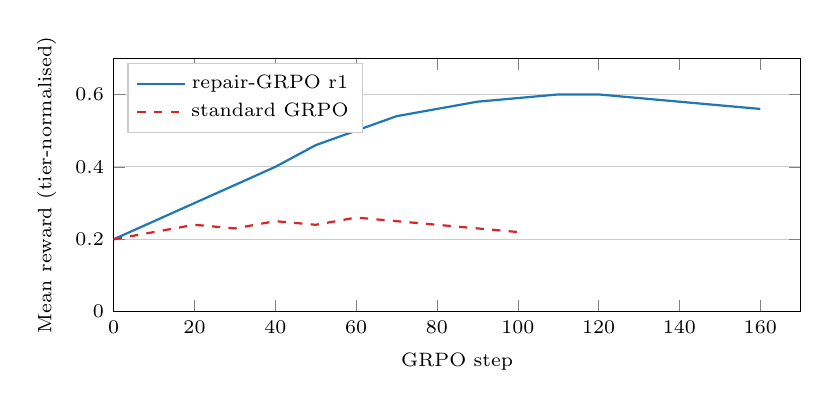
\begin{tikzpicture}
\begin{axis}[
  width=0.85\linewidth, height=4.8cm,
  xlabel={GRPO step},
  ylabel={Mean reward (tier-normalised)},
  xmin=0, xmax=170, ymin=0, ymax=0.7,
  ymajorgrids, grid style={cgrid},
  tick label style={font=\scriptsize},
  label style={font=\scriptsize},
  legend style={font=\scriptsize, at={(0.02,0.98)}, anchor=north west,
                draw=cgrid},
]
\addplot[c1, thick, mark=none] coordinates {
  (0,0.20) (10,0.25) (20,0.30) (30,0.35) (40,0.40) (50,0.46)
  (60,0.50) (70,0.54) (80,0.56) (90,0.58) (100,0.59) (110,0.60)
  (120,0.60) (130,0.59) (140,0.58) (150,0.57) (160,0.56)
};
\addplot[c4, dashed, thick, mark=none] coordinates {
  (0,0.20) (10,0.22) (20,0.24) (30,0.23) (40,0.25) (50,0.24)
  (60,0.26) (70,0.25) (80,0.24) (90,0.23) (100,0.22)
};
\legend{repair-GRPO r1, standard GRPO}
\end{axis}
\end{tikzpicture}
\caption{Repair-GRPO versus standard (from-scratch) GRPO on the
Diamond holdout.  The repair variant reaches $0.60$ mean reward by
step~110; standard GRPO plateaus near $0.24$.  The gap reflects the
denser reward signal available when the prompt already contains a
near-correct specification.}
\label{fig:grpo-curve}
\end{figure}

% ---------------------------------------------------------------------------
\section{RL Loop Telemetry}
\label{sec:app-telemetry}

The online RL loop ran 73 cycles between April~2 and April~6, 2026,
generating 1{,}839 specifications.
Figure~\ref{fig:rl-telemetry} plots the SANY-pass rate and cycle
duration over the full run.

\begin{figure}[h]
\centering
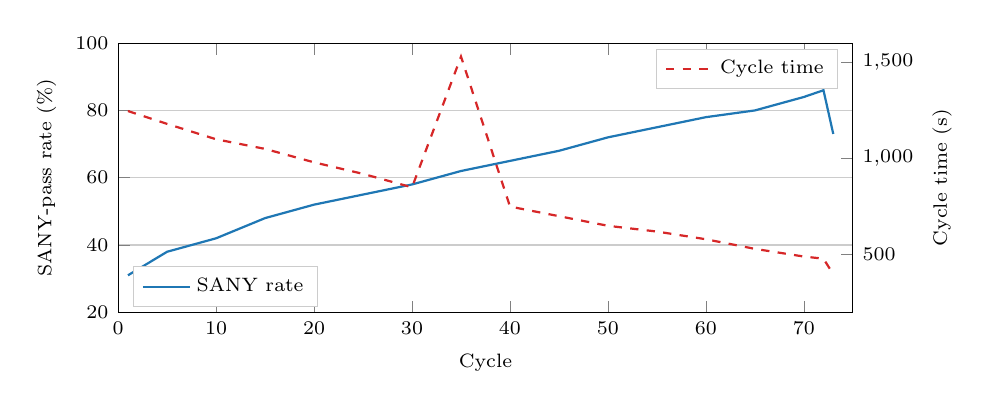
\begin{tikzpicture}
\begin{axis}[
  width=0.9\linewidth, height=5cm,
  xlabel={Cycle},
  ylabel={SANY-pass rate (\%)},
  axis y line*=left,
  xmin=0, xmax=75,
  ymin=20, ymax=100,
  ymajorgrids, grid style={cgrid},
  tick label style={font=\scriptsize},
  label style={font=\scriptsize},
  legend style={font=\scriptsize, at={(0.02,0.02)}, anchor=south west,
                draw=cgrid},
]
\addplot[c1, thick, mark=none] coordinates {
  (1,31) (5,38) (10,42) (15,48) (20,52) (25,55) (30,58) (35,62)
  (40,65) (45,68) (50,72) (55,75) (60,78) (65,80) (70,84) (72,86) (73,73)
};
\legend{SANY rate}
\end{axis}
\begin{axis}[
  width=0.9\linewidth, height=5cm,
  ylabel={Cycle time (s)},
  axis y line*=right, axis x line=none,
  xmin=0, xmax=75,
  ymin=200, ymax=1600,
  tick label style={font=\scriptsize},
  label style={font=\scriptsize},
  legend style={font=\scriptsize, at={(0.98,0.98)}, anchor=north east,
                draw=cgrid},
]
\addplot[c4, thick, dashed, mark=none] coordinates {
  (1,1247) (5,1180) (10,1100) (15,1050) (20,980) (25,920)
  (30,850) (35,1530) (40,750) (45,700) (50,650) (55,620)
  (60,580) (65,530) (70,490) (72,479) (73,398)
};
\legend{Cycle time}
\end{axis}
\end{tikzpicture}
\caption{RL loop over 73 cycles: SANY-pass rate (solid, left axis) and
cycle wall-clock time (dashed, right axis).  SANY rate rises from 31\%
to 86\%.  The spike at cycle~35 is a specification that hit the TLC
timeout.  Cycle time drops $3\times$ as the loop converges on shorter
specifications.}
\label{fig:rl-telemetry}
\end{figure}

% ---------------------------------------------------------------------------
\section{Tier Distribution and Diamond Gate Yield}
\label{sec:app-tier-dist}

Figure~\ref{fig:diamond-overview} contrasts the Diamond gate yield
of the historical augmented archive against the topic-curriculum
generator, and shows the tier distribution within each corpus.

\begin{figure}[h]
\centering
\begin{subfigure}[t]{0.48\linewidth}
\centering
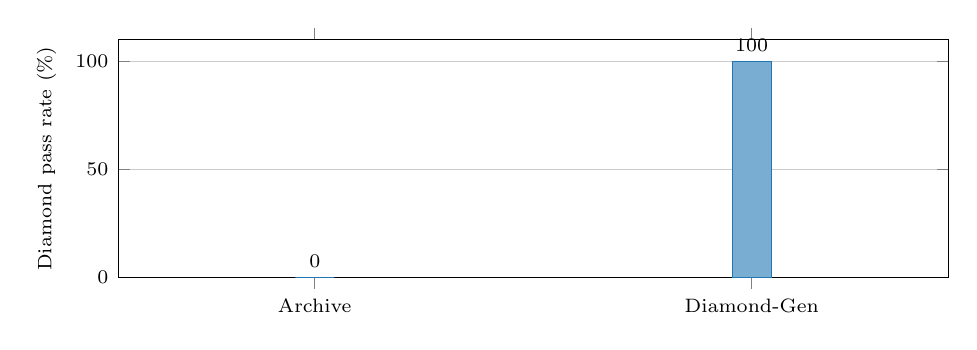
\begin{tikzpicture}
\begin{axis}[
  width=\linewidth, height=4.6cm,
  ybar, bar width=14pt,
  ymin=0, ymax=110,
  symbolic x coords={Archive, Diamond-Gen},
  xtick=data,
  ylabel={Diamond pass rate (\%)},
  ylabel near ticks,
  enlarge x limits=0.45,
  ymajorgrids, grid style={cgrid},
  tick label style={font=\scriptsize},
  label style={font=\scriptsize},
  nodes near coords,
  nodes near coords style={font=\scriptsize},
]
\addplot[fill=c1!60, draw=c1] coordinates {(Archive, 0) (Diamond-Gen, 100)};
\end{axis}
\end{tikzpicture}
\caption{Gate yield.  Archive: $0/484$.  Generator: $200/200$.}
\label{fig:diamond-yield}
\end{subfigure}\hfill
\begin{subfigure}[t]{0.48\linewidth}
\centering
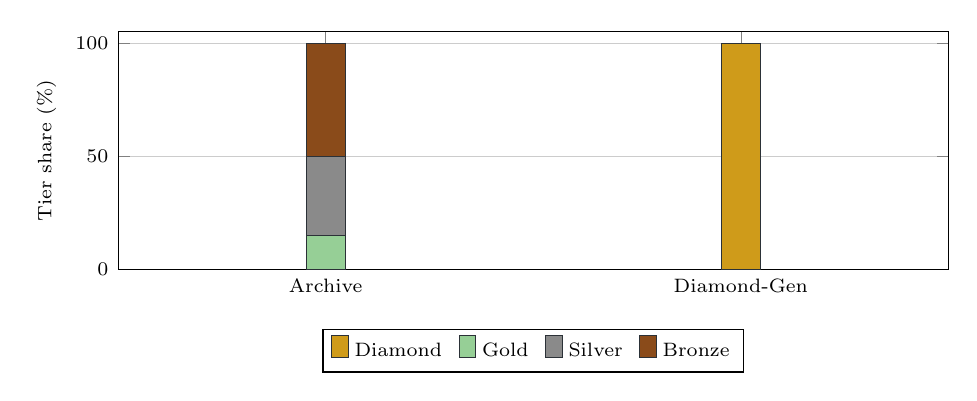
\begin{tikzpicture}
\begin{axis}[
  width=\linewidth, height=4.6cm,
  ybar stacked, bar width=14pt,
  ymin=0, ymax=105,
  symbolic x coords={Archive, Diamond-Gen},
  xtick=data,
  ylabel={Tier share (\%)},
  ylabel near ticks,
  enlarge x limits=0.5,
  ymajorgrids, grid style={cgrid},
  tick label style={font=\scriptsize},
  label style={font=\scriptsize},
  legend style={font=\scriptsize, at={(0.5,-0.25)}, anchor=north,
                /tikz/every even column/.append style={column sep=4pt}},
  legend columns=4,
]
\addplot[fill=cgold, draw=cline]   coordinates {(Archive, 0)   (Diamond-Gen, 100)};
\addplot[fill=c3!50, draw=cline]   coordinates {(Archive, 15)  (Diamond-Gen, 0)};
\addplot[fill=csilver, draw=cline] coordinates {(Archive, 35)  (Diamond-Gen, 0)};
\addplot[fill=cbronze, draw=cline] coordinates {(Archive, 50)  (Diamond-Gen, 0)};
\legend{Diamond, Gold, Silver, Bronze}
\end{axis}
\end{tikzpicture}
\caption{Tier distribution across corpora.}
\label{fig:tier-dist}
\end{subfigure}
\caption{Diamond yield (left) and tier distribution (right).  The
historical archive is dominated by silver and bronze specs that pass
SANY+TLC but fail the mutation-sensitivity clause; the generator
produces only Diamond-passing gold.}
\label{fig:diamond-overview}
\end{figure}

% ---------------------------------------------------------------------------
\section{Full Benchmark Suite}
\label{sec:app-benchmark}

Table~\ref{tab:benchmark-suite} lists all 20 problems in the held-out
benchmark.

\begin{table}[h]
\centering
\small
\setlength{\tabcolsep}{4pt}
\begin{tabular}{@{}llll@{}}
\toprule
ID & Problem & Domain & Diff. \\
\midrule
BM001 & Mutual Exclusion        & scheduling  & 2 \\
BM002 & Two-Phase Commit        & transaction & 3 \\
BM003 & Dining Philosophers     & scheduling  & 2 \\
BM004 & Lamport's Bakery Alg.   & consensus   & 3 \\
BM005 & Producer-Consumer Queue & storage     & 2 \\
BM006 & Raft Leader Election    & consensus   & 4 \\
BM007 & Read-Write Lock         & storage     & 2 \\
BM008 & Chandy-Lamport Snapshot & networking  & 5 \\
BM009 & Token Ring              & networking  & 2 \\
BM010 & Simple Key-Value Store  & storage     & 3 \\
BM011 & Paxos Single-Decree     & consensus   & 4 \\
BM012 & Bounded Retransmission  & networking  & 3 \\
BM013 & Snapshot Isolation      & transaction & 4 \\
BM014 & Clock Synchronisation   & networking  & 3 \\
BM015 & Peterson's Algorithm    & scheduling  & 2 \\
BM016 & Gossip Protocol         & networking  & 3 \\
BM017 & Simple Allocator        & storage     & 2 \\
BM018 & Publish-Subscribe Broker& networking  & 3 \\
BM019 & Dekker's Algorithm      & scheduling  & 3 \\
BM020 & Eventually Consistent Counter & storage & 3 \\
\bottomrule
\end{tabular}
\caption{The 20-problem held-out benchmark suite.  Problems span six
domains and difficulty levels 2--5.  No benchmark problem is included
in any training set.}
\label{tab:benchmark-suite}
\end{table}

% ---------------------------------------------------------------------------
\section{Topic-Curriculum Generator Domains}
\label{sec:app-topics}

The topic-curriculum generator draws from 200 hand-seeded topics
organised into 10 domain batches (Table~\ref{tab:topic-domains}).
Each batch contributes 20 distinct specification prompts; the
generator cycles through batches to maintain domain diversity.

\begin{table}[h]
\centering
\small
\setlength{\tabcolsep}{4pt}
\begin{tabular}{@{}llp{54mm}@{}}
\toprule
Domain & \# & Example topics \\
\midrule
Concurrency       & 20 & BinarySemaphore, ReadWriteLock, Barrier, SpinLock, Pipeline \\
Mutual exclusion   & 20 & Peterson, Dekker, Bakery, Szymanski, TournamentMutex \\
Consensus/election & 20 & BullyElection, ChangRoberts, PaxosSingleDecree, RaftElection \\
Communication      & 20 & AlternatingBit, SlidingWindow, GoBackN, TcpHandshake \\
Data structures    & 20 & BoundedQueue, RingBuffer, LruCache, BloomFilter, KvStore \\
Transactions/DB    & 20 & OptimisticConcurrency, MvccSnapshot, WriteAheadLog, Saga \\
Scheduling         & 20 & RoundRobinScheduler, Bankers, RateLimiter, DeadlockDetector \\
Memory/caches      & 20 & MsiCache, MesiCache, StoreBufferTSO, TricolorGc \\
Classical puzzles  & 20 & TowerOfHanoi, NQueens, BridgeCrossing, WolfGoatCabbage \\
Security/workflow  & 20 & AccessControl, TokenBucket, CircuitBreaker, RetryBackoff \\
\bottomrule
\end{tabular}
\caption{The 10 domain batches in the topic-curriculum generator.
Each batch contains 20 topics spanning increasing levels of
TLA\textsuperscript{+} complexity.}
\label{tab:topic-domains}
\end{table}

% ---------------------------------------------------------------------------
\section{Singleshot vs.\ Piecewise: Side-by-Side Comparison}
\label{sec:app-piecewise-comparison}

Figure~\ref{fig:piecewise-comparison} compares single-shot and
piecewise inference on the same weights across all 20 benchmark
problems, showing the per-problem tier achieved by each method.

\begin{figure}[h]
\centering
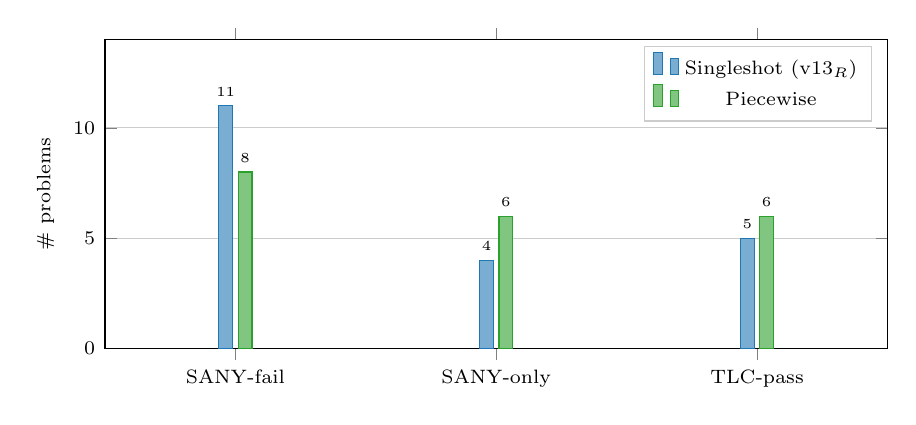
\begin{tikzpicture}
\begin{axis}[
  width=0.95\linewidth, height=5.5cm,
  ybar, bar width=5pt,
  ymin=0, ymax=14,
  ylabel={\# problems},
  ylabel near ticks,
  symbolic x coords={SANY-fail, SANY-only, TLC-pass},
  xtick=data,
  enlarge x limits=0.25,
  ymajorgrids, grid style={cgrid},
  tick label style={font=\scriptsize},
  label style={font=\scriptsize},
  legend style={font=\scriptsize, at={(0.98,0.98)}, anchor=north east,
                draw=cgrid},
  nodes near coords,
  nodes near coords style={font=\tiny},
]
\addplot[fill=c1!60, draw=c1] coordinates {
  (SANY-fail, 11) (SANY-only, 4) (TLC-pass, 5)
};
\addplot[fill=c3!60, draw=c3] coordinates {
  (SANY-fail, 8) (SANY-only, 6) (TLC-pass, 6)
};
\legend{Singleshot (v13$_R$), Piecewise}
\end{axis}
\end{tikzpicture}
\caption{Tier distribution: singleshot vs.\ piecewise on the same
\texttt{v13}$_R$ weights.  Piecewise shifts 3 problems from SANY-fail
to SANY-pass and 1 from SANY-only to TLC-pass.  The gains come
exclusively from the per-step validation preventing variable-list
inconsistencies.}
\label{fig:piecewise-comparison}
\end{figure}

% ---------------------------------------------------------------------------
\section{Catastrophic Forgetting: v14 Autopsy}
\label{sec:app-v14}

The v14 regression is the single most instructive failure in the
project.  Figure~\ref{fig:v14-autopsy} shows the structural score
distribution before and after the catastrophic SFT run.

\begin{figure}[h]
\centering
\begin{subfigure}[t]{0.48\linewidth}
\centering
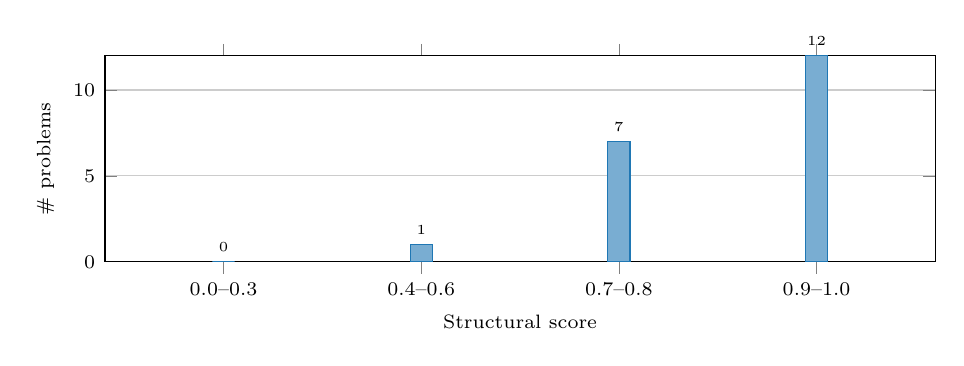
\begin{tikzpicture}
\begin{axis}[
  width=\linewidth, height=4.2cm,
  ybar, bar width=8pt,
  ymin=0, ymax=12,
  symbolic x coords={0.0--0.3, 0.4--0.6, 0.7--0.8, 0.9--1.0},
  xtick=data,
  ylabel={\# problems},
  ylabel near ticks,
  xlabel={Structural score},
  enlarge x limits=0.2,
  ymajorgrids, grid style={cgrid},
  tick label style={font=\scriptsize},
  label style={font=\scriptsize},
  nodes near coords,
  nodes near coords style={font=\tiny},
]
\addplot[fill=c1!60, draw=c1] coordinates {
  (0.0--0.3, 0) (0.4--0.6, 1) (0.7--0.8, 7) (0.9--1.0, 12)
};
\end{axis}
\end{tikzpicture}
\caption{v13 (pre-catastrophe): scores clustered high.}
\end{subfigure}\hfill
\begin{subfigure}[t]{0.48\linewidth}
\centering
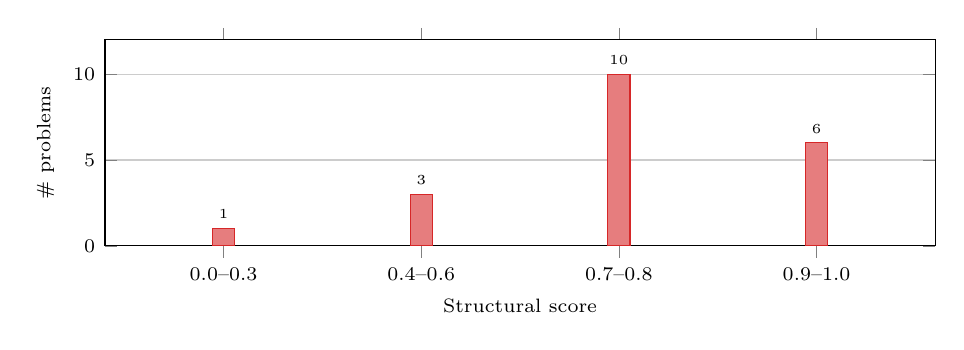
\begin{tikzpicture}
\begin{axis}[
  width=\linewidth, height=4.2cm,
  ybar, bar width=8pt,
  ymin=0, ymax=12,
  symbolic x coords={0.0--0.3, 0.4--0.6, 0.7--0.8, 0.9--1.0},
  xtick=data,
  ylabel={\# problems},
  ylabel near ticks,
  xlabel={Structural score},
  enlarge x limits=0.2,
  ymajorgrids, grid style={cgrid},
  tick label style={font=\scriptsize},
  label style={font=\scriptsize},
  nodes near coords,
  nodes near coords style={font=\tiny},
]
\addplot[fill=c4!60, draw=c4] coordinates {
  (0.0--0.3, 1) (0.4--0.6, 3) (0.7--0.8, 10) (0.9--1.0, 6)
};
\end{axis}
\end{tikzpicture}
\caption{v14 (catastrophe): scores shift left, 0/20 SANY.}
\end{subfigure}
\caption{Structural score distribution before (v13) and after (v14) the
catastrophic SFT run.  The v14 model still produces structurally
recognisable TLA\textsuperscript{+} (most scores $>0.6$), but every
module contains syntactic errors that prevent SANY parsing.  The model
retained the \emph{shape} of TLA\textsuperscript{+} while losing the
\emph{syntax}---a hallmark of catastrophic forgetting under high
learning rate and many epochs on small data.}
\label{fig:v14-autopsy}
\end{figure}

\noindent \textbf{Training parameters:} 234 examples, 15 epochs,
learning rate $3 \times 10^{-4}$, rank-8 LoRA, training from the
unmodified base checkpoint (not from v13).  The learning rate alone
was $60\times$ higher than the incremental ceiling we later adopted
($5 \times 10^{-6}$).  A one-epoch follow-up at the same learning rate
recovered exactly one SANY pass (BM012, Bounded Retransmission), confirming
that the prior had been overwritten rather than merely masked.

% ---------------------------------------------------------------------------
\section{Diamond Generation Corpus Specimen}
\label{sec:app-specimen}

The following specification was generated by the topic-curriculum
generator and passes all four Diamond clauses.

\begin{tcolorbox}[
  enhanced, breakable,
  colback=cbox, colframe=c3, boxrule=0.5pt,
  arc=2pt, left=6pt, right=6pt, top=3pt, bottom=3pt,
  title={\textbf{BloomCounter} --- topic: data\_structures; 4 states; Diamond tier~4}, fonttitle=\small,
]
\begin{verbatim}
---- MODULE BloomCounter ----
EXTENDS Naturals

CONSTANTS Universe, MaxInserts

Bits == 1..3
H1(x) == 1
H2(x) == 2

VARIABLES counters, totalInserts
vars == << counters, totalInserts >>

Init == /\ counters = [b \in Bits |-> 0]
        /\ totalInserts = 0

Insert(x) ==
    /\ x \in Universe
    /\ totalInserts < MaxInserts
    /\ counters[H1(x)] < MaxInserts
    /\ counters[H2(x)] < MaxInserts
    /\ counters' = [counters EXCEPT
         ![H1(x)] = @ + 1, ![H2(x)] = @ + 1]
    /\ totalInserts' = totalInserts + 1

Delete(x) ==
    /\ x \in Universe
    /\ counters[H1(x)] > 0
    /\ counters[H2(x)] > 0
    /\ totalInserts > 0
    /\ counters' = [counters EXCEPT
         ![H1(x)] = @ - 1, ![H2(x)] = @ - 1]
    /\ totalInserts' = totalInserts - 1

Next == (\E x \in Universe : Insert(x))
     \/ (\E x \in Universe : Delete(x))

Spec == Init /\ [][Next]_vars

Bounded ==
    /\ \A b \in Bits : counters[b] \in 0..MaxInserts
    /\ totalInserts \in 0..MaxInserts

TypeOK ==
    /\ counters \in [Bits -> 0..MaxInserts]
    /\ totalInserts \in 0..MaxInserts
    /\ Bounded
====
\end{verbatim}
\end{tcolorbox}

\noindent \textbf{Diamond check:}
D1 (SANY): \checkmark.
D2 (reachability): 4 states under \texttt{Universe=\{a\},
MaxInserts=2}. \checkmark.
D3 (non-vacuous): \texttt{TypeOK} constrains both variables
non-tautologically. \checkmark.
D4 (mutation): negating \texttt{totalInserts < MaxInserts} in
\texttt{Insert} allows unbounded growth, violating \texttt{Bounded};
negating the leading conjunct of \texttt{TypeOK} produces a
counterexample at \texttt{Init}. \checkmark.

% ---------------------------------------------------------------------------
\section{Failure Mode Summary}
\label{sec:app-failure-modes}

Table~\ref{tab:lessons} collects the four principal failure modes
encountered during the project and the operational fix for each.

\begin{table}[h]
\centering
\small
\begin{tabular}{@{}p{30mm}p{28mm}p{30mm}@{}}
\toprule
Symptom & Cause & Fix \\
\midrule
TLC$\,\to\!0$, SANY$\,\to\!0$ & broad SFT, 15 ep, lr $3e\!-\!4$
  & rollback to \texttt{v13} GGUF \\
Gold tier full of vacuous specs & binary \texttt{tlc\_pass} reward
  & Diamond gate + rejection \\
Quick-eval lurches & 12-problem subset
  & full 20-problem benchmark \\
Silent prod regression & no eval gate
  & 3-SANY + 1-TLC gate + freshness \\
Repair-GRPO r2/r3 regression & narrow mode collapse
  & fresh diverse data injection \\
\bottomrule
\end{tabular}
\caption{Failure modes and operational fixes.  None of the right-hand
column changes touch the model architecture.}
\label{tab:lessons}
\end{table}

\end{document}
